%-------------------------------------------------------------------------------
% FIELD ADVANTAGES
%-------------------------------------------------------------------------------
\subsection{Field advantages}
\begin{frame}{Application: game modeling}{Field advantages}

\begin{figure}[ht]
\begin{minipage}[t]{0.5\linewidth}
\vspace{0pt}
\begin{block}{Strategic game play}
\begin{itemize}
\item A good test of cognition,
\item easy performance evaluation,
\item a well documented problem.
\end{itemize}
\end{block}
\end{minipage}
\hfill
\begin{minipage}[t]{0.4\linewidth}
\vspace{0pt}
\centering
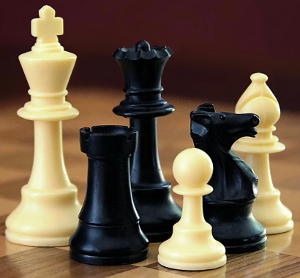
\includegraphics[width=\textwidth]{img/application/chess.png}
\end{minipage}
\end{figure}

\end{frame}

%-------------------------------------------------------------------------------
% CHOSEN GAME: "REVERSI"
%-------------------------------------------------------------------------------
\subsection{Chosen game: ``Reversi"}
\begin{frame}{Application: game modeling}{Chosen game: ``Reversi"}

\begin{figure}[ht]
\begin{minipage}[t]{0.4\linewidth}
\vspace{0pt}
\centering
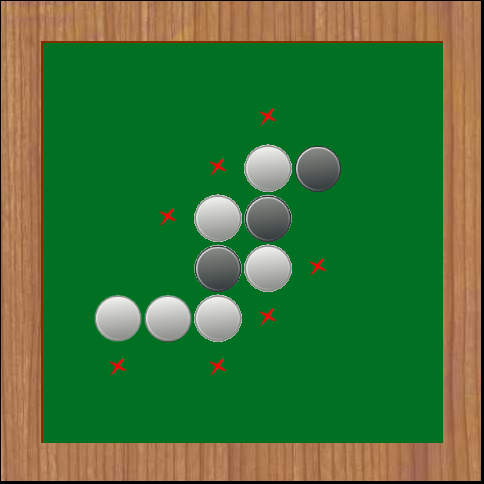
\includegraphics[width=\textwidth]{img/application/reversi.png}
\end{minipage}
\hfill
\begin{minipage}[t]{0.5\linewidth}
\vspace{0pt}
\begin{block}{Basic idea}
\begin{itemize} 
\item Place coloured pieces,
\item convert the opponents',
\item have more pieces at the end.
\end{itemize}
\end{block}
\end{minipage}

\end{figure}

\end{frame}

%-------------------------------------------------------------------------------
% VON NEUMANN'S THEOREM
%-------------------------------------------------------------------------------
\subsection{Von Neumann's theorem}
\begin{frame}{Application: game modeling}{Von Neumann's theorem}
\begin{block}{``I cut, you choose"}
\centering
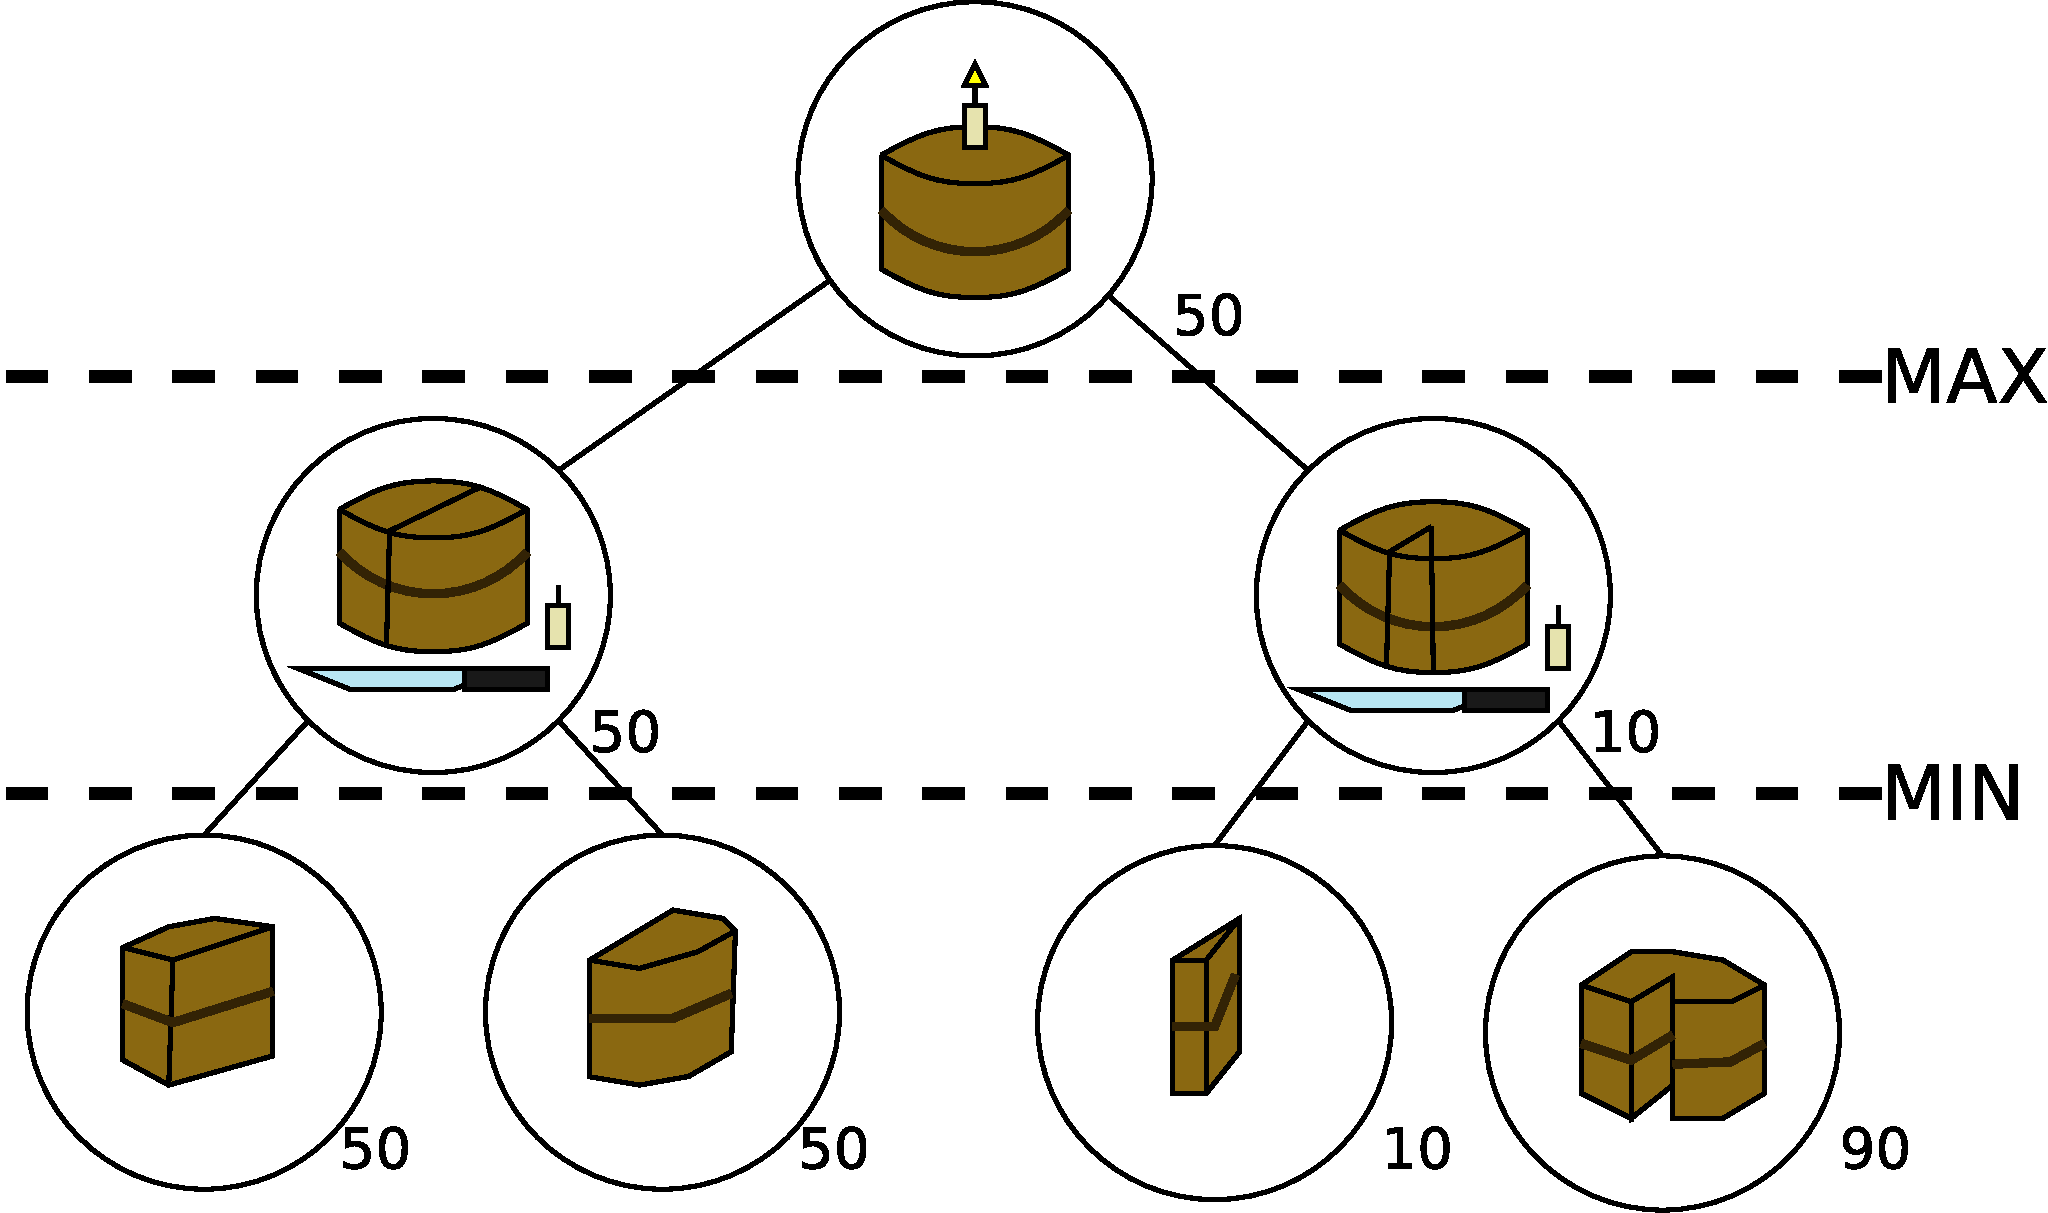
\includegraphics[height=0.6\paperheight]{img/application/cakes.pdf}
\end{block}
\end{frame}

%-------------------------------------------------------------------------------
% DRAWBACKS OF MINIMAX
%-------------------------------------------------------------------------------
\subsection{Drawbacks of Minimax}
\begin{frame}{Application: game modeling}{Drawbacks of Minimax}

\begin{block}{Exponential-time algorithm}
\begin{itemize}
\item Search-depth must be capped,
\item heuristics must be used,
\item theoretical optimality is lost.
\end{itemize}
\end{block}

\begin{block}{``Multum in parvo"}
It's difficult to condense expert knowledge into a heuristic!
\end{block}

\end{frame}

%-------------------------------------------------------------------------------
% AN ALTERNATIVE
%-------------------------------------------------------------------------------
\subsection{An alternative}
\begin{frame}{Application: game modeling}{An alternative}

\huge{Why not have the system develop its own heuristic through trial and error?}

\end{frame}